% ------------------------------------------------------------------------
% Name: Introduction
% Author: Emmanuel SCHWARTZ
% Date: November 2016
% Description: Introduction Chapter for my master thesis paper
% ------------------------------------------------------------------------

\section{Motivation}
\textbf{!!!!!! find catch phrase as intro !!!!!! }
Last downside of e-mails involves the user. Nowadays, it is common practice to send business documents via e-mail or via supplier\textquoteright s web portal: Faster and cheaper compared to a hard copy sent via post. But, how can a user successuffly order and sort out differents kinds of documents, coming from different mailboxes? In most cases, the user does not have a clue how to establish a \textbf{document management}: local storage? cloud storage? And what if the computer has hard drive failures, or is infected by viruses: Did they make regular back-ups?
\paragraph{}
With respect to the application senario described in the next section, this thesis will try to answer these problems with new upcoming technologies such as blockchains, decentralized storage and Dapps. 
 
\section {Application Scenario}
\paragraph{}
 Even if the big actors of Internet are trying to adapt e-mails to nowadays requirements, e-mails might not be the right solution anymore to send buisiness documents. Figure 1.1 shows the path that an e-mail takes to go from the company to a client, jumping through servers via the protocol SMTP. Once the email has eached the client's mail server, the client has the choice to synchronize his email between 3 protocols: IMAP, POP3 or SMTP.
\begin{figure}[htp]
\centering
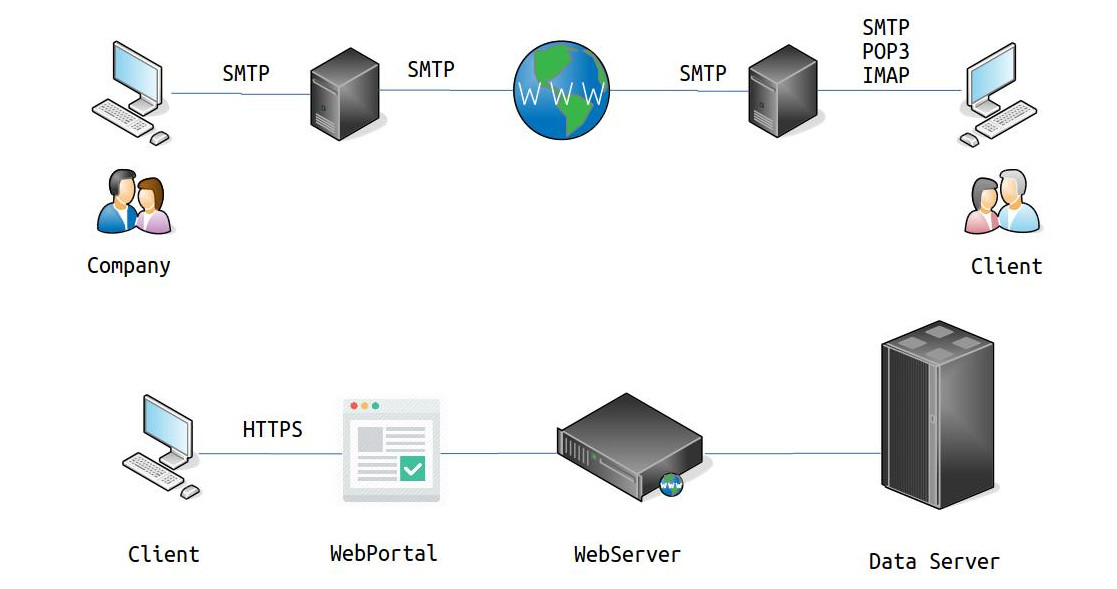
\includegraphics[scale=0.49]{/home/emmanuel/Documents/masterThesis/doc/ressources/email&webportal.jpg}
\caption{}
\label{}
\end{figure}
\newline
New technologies that Bitcoin has brought, paired up with decentralized storage providers, can revolutionize the way we are going to send documents, described in the figure 1.2. 
\begin{figure}[htp]
\centering
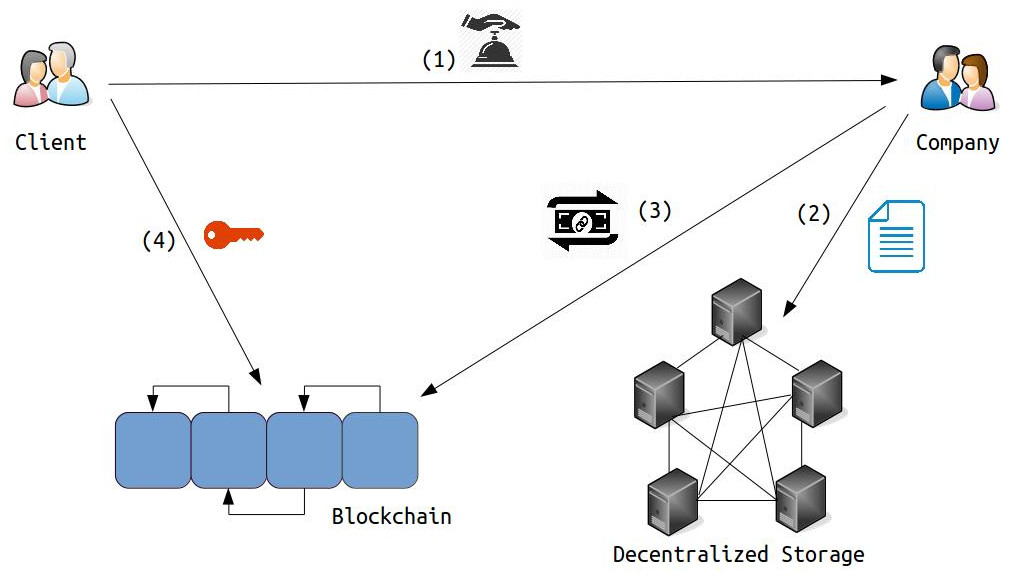
\includegraphics[scale=0.47]{/home/emmanuel/Documents/masterThesis/doc/ressources/blockchain.jpg}
\caption{}
\label{}
\end{figure}
\newline
The customer is creating a request to the company for a specific document (1). Then, the document is stored using a distributed storage provider (2). A link is created, which is stored directly in the blockchain by doing an transaction (3). The blockchain transaction provides the evidence, that the document has been sent and keeps a permanent not alterable link to the document. In order to open a document, the customer only needs its private key (4). (For further explanation, see 2.2)

\section{Objective}
\paragraph{}
The main goal of this thesis is to see if there is a possible implementation of a proof of concept (poc) using the new technologies such as blockchains, decentralized storage and Dapps to send documents between a company and a customer. Pros and Cons will be also discussed. Additionnally, MetaData can give useful information such as the author of a document, the timestamp, some comments etc etc. This thesis will show if metadata can be added during a transaction. Besides these constraints, a document should be also signed Within the proposed architecture. Furthermore, a flexible approach is desirable that supports multiple storage providers such as Amazon, Azure, IPFS, StorJ. Last but not least, this implemantation should be able to be combined with traditional cloud systems.
\newline
In summary, the objective is to find a proof of concept that can send documents between two users with the following points:
\begin{easylist}[enumerate]
\ListProperties(Hide=100, Hang=false, Progressive=3ex, Style*=--)
& A dvantages and limitations of this architecture
& Signing a document with this architecture?
& Combination with traditional cloud systems
& Flexible regarding storage providers
& Easy \& intuitive GUI for users
& Metadata
\end{easylist}

\section{Overview}
\paragraph{}
\textbf{!!!!!!!!!!!!!!!!!!!!!!!! TBD !!!!!!!!!!!!!!!!!!!}
To achieve the objectives stated in section 1.3, chapter 2 - Related Work and Basic Principles - contains an in-depth overview of state of the decentralized document management.
TDB: 2.1, 2.2, 2.3 etc
Chapter 3 presents the method.
Chapter 4: evaluate the proposed approaches  
Finally, chapter 5 concludes the work %and highlights the applicability of the developed approaches to other domains. 
